\section{Experimental evaluation}\label{sec:experimental-evaluation}

\subsection{Experiment setup}

\subsubsection{Datasets}

The proposed methods were experimentally verified on several datasets. The datasets Cora and CiteSeer \cite{yang_revisiting_2016} were used with the \enquote{full} train-test split as in \cite{chen_fastgcn_2018}. Two larger datasets were also used, the PubMed dataset \cite{yang_revisiting_2016} and the DBLP dataset \cite{bojchevski_deep_2018}. In addition, 6 variants of the Twitch dataset \cite{rozemberczki_multi-scale_2021} were used. The basic properties of these datasets are listed in Table~\ref{tab:dataset-sizes}.

\begin{table*}
  \begin{center}
    \begin{minipage}{280pt} % Tune this when the table is changed using the lua-visual-debug package
      \caption{Basic properties of the used datasets}
      \label{tab:dataset-sizes}
      \begin{tabular}{lrrrr}
        \toprule
        \textbf{Dataset} & \textbf{Nodes} & \textbf{Edges} & \textbf{Node features} & \textbf{Classes} \\
        \midrule
        Cora             & 2 708          & 10 556         & 1 433                  & 7                \\
        CiteSeer         & 3 327          & 9 104          & 3 703                  & 6                \\
        PubMed           & 19 717         & 88 648         & 500                    & 3                \\
        DBLP             & 17 716         & 105 734        & 1 639                  & 4                \\
        Twitch-DE        & 9 498          & 315 774        & 128                    & 2                \\
        Twitch-EN        & 7 126          & 77 774         & 128                    & 2                \\
        Twitch-ES        & 4 648          & 123 412        & 128                    & 2                \\
        Twitch-FR        & 6 551          & 231 883        & 128                    & 2                \\
        Twitch-PT        & 1 912          & 64 510         & 128                    & 2                \\
        Twitch-RU        & 4 385          & 78 993         & 128                    & 2                \\
        \bottomrule
      \end{tabular}
    \end{minipage}
  \end{center}
\end{table*}

\subsubsection{Methodology of experiments}

The hyper-parameters for both the node2vec model used for the embedding training and the multi-layer perceptron used for downstream classification were initially set to values used in prior art (see \cite{hu_open_2021, fey_fast_2019}) and then manually fine-tuned for each dataset.

The achitecture of the algorithm was identical accross the dataset, with the only difference being in the values of the hyper-parameters, as listed in Table~\ref{tab:hyperparameter-values}. For the Cora dataset, the node2vec model generated an embedding in \( \mathfield{R}^{128} \) from \( 4 \) random walks of length \( 20 \) for each node with a context window of size \( 5 \). The optimizer ADAM \cite{kingma_adam:_2017} was used with a learning rate of \( 0.01 \) and batches of \( 128 \) samples. The model was trained for \( 5 \) epochs and in each step of the adaptive prolongation, \( 100 \) nodes were prolonged, until reaching the original graph. The MLP classifier using the embeddings featured \( 3 \) linear layers of \( 128 \) neurons with batch normalization after each layer. Each layer was normalized using dropout \cite{srivastava_dropout_2014} with the rate of \( 0.5 \). Finally, a linear layer was used for the class prediction. For the classifier, ADAM with a learning rate of \( 0.01 \) was used for \( 30 \) epochs of training with the cross-entropy loss function. Dataset features weren't used for the classifier training as the aim of this work is to compare the embeddings. The experiment was run \( 10 \) times end-to-end and results averaged. The experiments were implemented using PyTorch \cite{paszke_pytorch_2019} and PyTorch Geometric \cite{fey_fast_2019}.

\begin{table*}
  \begin{center}
    \begin{minipage}{360pt} % Tune this when the table is changed using the lua-visual-debug package
      \caption{Hyper-parameter values used for different datasets}
      \label{tab:hyperparameter-values}
      \begin{tabular}{lrrrrr}
        \toprule
        \textbf{Hyper-parameter} & \textbf{Cora} & \textbf{CiteSeer} & \textbf{PubMed} & \textbf{DBLP} & \textbf{Twitch} \\
        \midrule
        Embedding dimension      & 128           & 32                & 64              & 32            & 128             \\
        \# of random walks       & 4             & 5                 & 3               & 2             & 10              \\
        Random walk length       & 20            & 20                & 40              & 20            & 80              \\
        Context window size      & 5             & 5                 & 20              & 5             & 3               \\
        Node2vec learning rate   & 0.01          & 0.01              & 0.01            & 0.01          & 0.025           \\
        Node2vec batch size      & 128           & 128               & 128             & 128           & 128             \\
        Node2vec epochs          & 5             & 7                 & 1               & 1             & 5               \\
        \# of prolonged nodes    & 100           & 150               & 1000            & 800           & 200             \\
        \# of MLP layers         & 3             & 3                 & 1               & 3             & 2               \\
        MLP hidden layer width   & 128           & 256               & 128             & 256           & 64              \\
        Dropout rate             & 0.5           & 0.5               & 0.5             & 0.5           & 0.5             \\
        MLP learning rate        & 0.01          & 0.01              & 0.01            & 0.01          & 0.01            \\
        MLP epochs               & 30            & 80                & 300             & 300           & 500             \\
        \bottomrule
      \end{tabular}
    \end{minipage}
  \end{center}
\end{table*}

\subsection{Evaluation of the adaptive approach}\label{sec:adaptive-experiments}

In order to study the effect of the adaptive prolongation, the adaptive prolongation method was used to assess the performance of downstream transductive classification at different coarsening levels. A node2vec model as described in the previous section was trained with adaptive prolongation based on coarsenings pre-computed by the HARP coarsening algorithm as described in \ref{sec:harp-coarsening}. For each prolongation step, the intermediary embedding was afterwards fully prolonged to obtain an embedding of the original graph \( G \) (as that is the only graph for which ground-truth labels are available). A classifier was then trained with this embedding as input. This setup allows us to compare classification accuracy at each step of the adaptive prolongation. Figure~\ref{fig:adaptive-coarsening} shows the results of this experiment, compared with a baseline node2vec model (that is, without any coarsening or prolongation) that was trained for the same number of epochs as the total epochs of the adaptive model over all prolongation steps.

\begin{figure*}
  \centering
  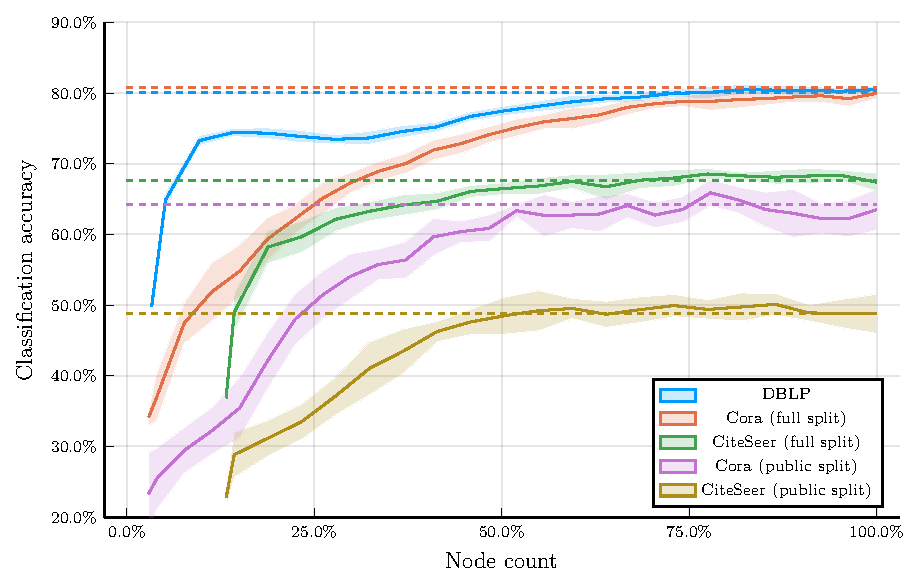
\includegraphics[width = \linewidth]{images/adaptive-coarsening/adaptive-coarsening.pdf}
  \caption{Downstream classifier accuracies at different steps of adaptive prolongation using the basic HARP coarsening algorithm. Dashed line shows the baseline node2vec model accuracy. The node count is taken relative to the total node count in each dataset. The results are averaged over multiple runs, with the solid line representing the mean and the shaded area denoting one standard deviation.}
  \label{fig:adaptive-coarsening}
\end{figure*}

The behaviour of the model somewhat differs between the used datasets. For the Cora, CiteSeer, DBLP and PubMed datasets, the model starts from a very low performance, which quickly rises as the model trains for several prolongation steps. The model trained on CiteSeer attains performance comparable to the reference model when approximately half of all nodes are available to it. On the other hand, with Cora, the model slowly approaches the reference model for the whole duration of training, only reaching comparable performance at a point where nearly the whole graph is available to it. Models trained on the two larger datasets, DBLP and PubMed, exhibit a different behaviour in that they briefly reach a global maximum followed by a slight decrease in performance until finally approaching the performance of the reference model in a manner similar to the models trained on Cora and CiteSeer. This behaviour is further discussed in the next section. The Twitch dataset is substantially different, with very high initial performance and only small performance gains with increasing number of nodes available, with different variants of it exhibiting this effect to a different magnitude.

To further study the model properties from a statistical point of view, the results were evaluated at \( k \)-th deciles of the node count of the full graph, for all possible values of \( k \). At each decile, the performance of the model was compared to the baseline node2vec model using the Wilcoxon signed-rank test with the Holm-Bonferroni correction for multiple hypothesis testing. The hypotheses were tested on all datasets.
%TODO: Holm-corrected Wilcoxons

Following recent best-practice recommendations regarding verifying the statistical validity of results \cite{benavoli_time_2017}, the results were also studied from the point of view of Bayesian estimation. Similarly to the frequentist approach, the performance of the model was compared to that of the baseline model at \( k \)-th deciles of the node count, for all possible values of \( k \). The comparison was done using the Bayesian Wilcoxon signed-rank test \cite{benavoli_bayesian_2014} for 3 different widths of the region of practical equivalence (ROPE), 1\%, 5\% and 10\%. The probabilities that the two models are practically equivalent are listed in Table~\ref{tab:bayesian-adaptive}. Of a particular note is the fact that at 50\% complexity, the models have over a 95\% probability of being within 5 percentage points of performance -- showing that the proposed method may offer a significant complexity reduction in exchange for a relatively minor decrease in performance.

\begin{table}
  \begin{center}
    \begin{minipage}{210pt} % Tune this when the table is changed using the lua-visual-debug package
      \caption{The probabilities that the adaptive approach will be practically equivalent to node2vec when compared on different fractions of the full graph and with different widths of the region of practical equivalence.}
      \label{tab:bayesian-adaptive}
      \begin{tabular}{lrrr}
        \toprule
        \textbf{Nodes} & \textbf{1\% ROPE} & \textbf{5\% ROPE} & \textbf{10\% ROPE} \\
        \midrule
        10\%                & 0.1\%             & 29.1\%            & 57.8\%             \\
        20\%                & 0.2\%             & 39.0\%            & 90.5\%             \\
        30\%                & 0.1\%             & 54.5\%            & 98.6\%             \\
        40\%                & 0.1\%             & 71.0\%            & 100.0\%            \\
        50\%                & 0.9\%             & 95.2\%            & 100.0\%            \\
        60\%                & 8.5\%             & 99.8\%            & 100.0\%            \\
        70\%                & 32.6\%            & 100.0\%           & 100.0\%            \\
        80\%                & 62.1\%            & 100.0\%           & 100.0\%            \\
        90\%                & 67.4\%            & 100.0\%           & 100.0\%            \\
        100\%               & 83.9\%            & 100.0\%           & 100.0\%            \\
        \bottomrule
      \end{tabular}
    \end{minipage}
  \end{center}
\end{table}

\subsection{The relationship of the results and the properties of the graph}

When the models for DBLP and PubMed are studied more closely, both reach a local maximum at around 14\% of the graph, followed by a slight decline and gradual approach to the baseline. This suggests a global structure in the data, which the model learns at the point of the local maxima. To investigate this hypothesis, several graph metrics were applied to the graphs generated during the adaptive prolongation algorithm run. All of the metrics were applied in two scenarios -- \enquote{absolute}, where the metric was applied to the graph at a particular step in the prolongation process, and \enquote{incremental}, where the metric was applied to the graph induced by the edge set \( \mathspace{C} \), that is, the set of edges to be contracted at that step.

The metrics used were:
\begin{itemize}
  \item Edge homophily \cite{zhu_beyond_2020} is the fraction of edges connecting nodes of the same class.
  \item Node homophily \cite{pei_geom-gcn_2020} is the fraction of node neighbours having the same class as the node in question, averaged over all nodes.
  \item Class homophily \cite{lim_large_2021} is a variant of node homophily that attempts to modify it in such a way as to make it invariant to the number of classes. The metric measures excess node homophily when compared to a null model where edges are independent of node labels.
  \item Adjusted homophily \cite{platonov_characterizing_2022} is a modification of edge homophily targeted at ensuring it is not not biased towards particular class size distributions and that the metric has a constant maximum attained only for perfectly homophilous graphs.
  \item Balanced accuracy \cite{platonov_characterizing_2022} is a modification of edge homophily that balances each classes' contribution.
  \item Adjusted accuracy \cite{platonov_characterizing_2022} is a modification of balanced accuracy aimed at ensuring a constant baseline.
  \item Label informativeness \cite{platonov_characterizing_2022} is a measure of the influence of a node's neighbours' classes to the label of the node itself.
  \item Global assortativity \cite{newman_mixing_2003} is a measure of the tendency of nodes to connect with other similar nodes, rather than dissimilar nodes.
\end{itemize}

The values of these metrics at different steps of the adaptive prolongation algorithm are shown in Figure~\ref{fig:metrics}.

\begin{figure*}
  \centering
  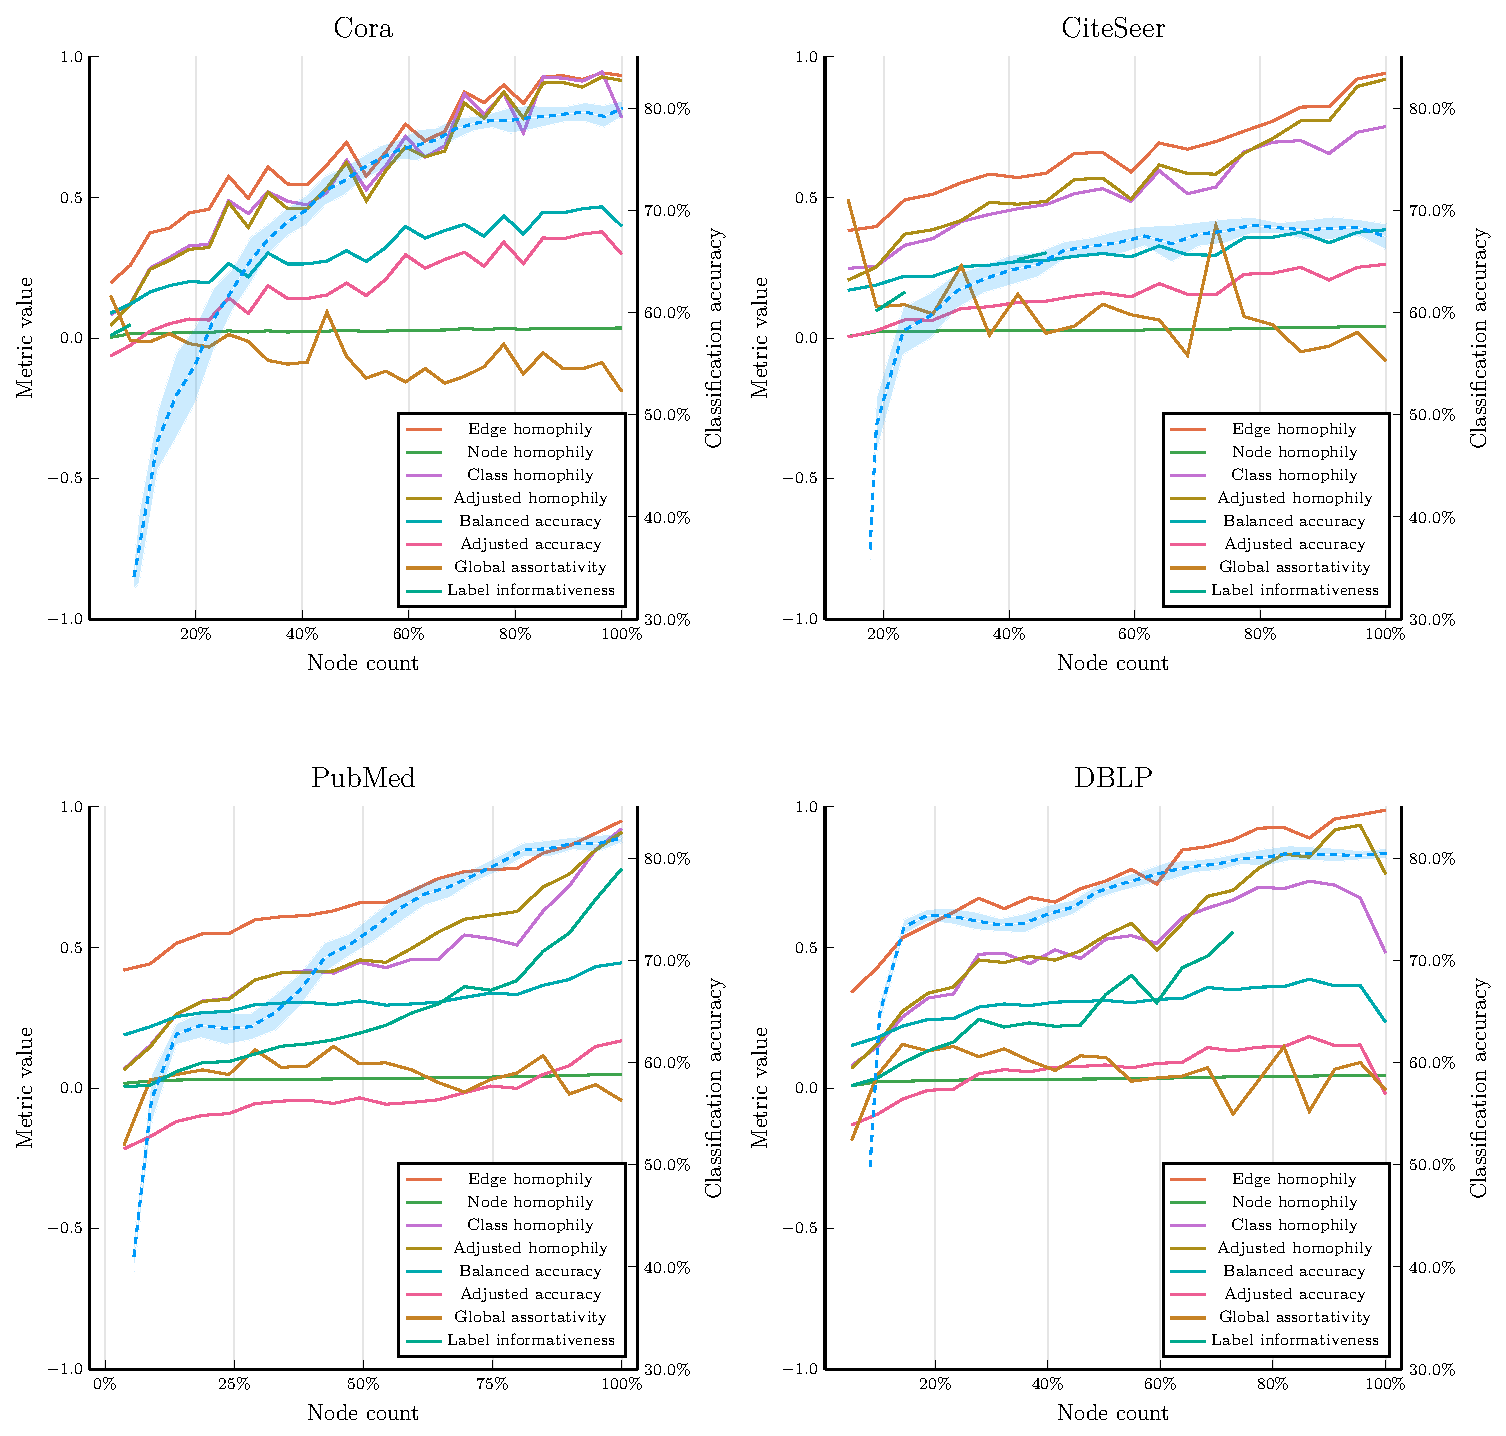
\includegraphics[width = \linewidth]{images/metrics/metrics.pdf}
  \caption{Values of the metrics for different datasets at different steps of the adpative prolongation algorithm. Overlaid as the dashed line is the accuracy of the downstream classifier.}
  \label{fig:metrics}
\end{figure*}

\subsection{Comparison of coarsening approaches}

For GDC coarsening, only the top-\( k \) sparsification method produces reliable results as thresholding leads to instability in the coarsening process, either collapsing the whole graph almost immediately, or not collapsing it at all. As for the other parameters, we followed \cite{gasteiger_diffusion_2019}. Both of the diffusion methods propsed in \cite{gasteiger_diffusion_2019} were implemented with the recommended parameter values, that is the heat kernel was used with the diffusion time \( t = 5 \) and the Personalized PageRank algorithm with the teleport probability \( \alpha = 0.15 \) and the recommended normalization. To be able to compute graph diffusion for larger graphs, approximate diffusion algorithms were used. For PPR, a version of the Andersen algorithm \cite{andersen_local_2006} with \( \epsilon = 10^{-2} \) was used and for heat kernel diffusion, a version of the Kloster-Gleich algorithm \cite{kloster_heat_2014} with \( \epsilon = 10^{-5} \) was used. Both of these algorithms were modified to produce edge weights as part of their output.

For the evolutionary coarsening, the experimental evaluation was conducted with crossover probability \( p_\mathrm{cx} = 0.9 \), individual and gene mutation probabilities \( p_\mathrm{mut} = p_\mathrm{gene} = 0.1 \), parent population size \( \lambda = 3 \), tournament size \( n_\mathrm{tourn} = 3 \), and the individual length \( L \) set to \( 5\% \) of the input graph node count. Each individual was evaluated \( 3 \) times and the results averaged to account for randomness in the evaluation. The set \( \mathspace{AC} \) consisted of 17 atomic coarsenings (Table~\ref{tab:atomic-coarsenings}), where the identity function is limited to maximally be 10\% of the individual. Only four of them had hyper-parameters. These were initialized by random sampling where \( d_\mathrm{lower} \) and \( d_\mathrm{upper} \) were sampled from a Poisson distribution with \( \mu = 30 \) and \( k \) and \( l \) were sampled uniformly from the set of all features. The evolution involved a maximum of 100 generations with an early stopping criterion triggering if the accuracy doesn't change more than 1\% in 10 generations. The evolutionary coarsening algorithm was implemented in the DEAP framework \cite{fortin_deap_2012}.

\begin{table*}
  \begin{center}
    \begin{minipage}{\textwidth}
      \caption{The atomic coarsening functions. In all atomic coarsenings, the edge is selected randomly in case of a tie in the condition.}
      \label{tab:atomic-coarsenings}
      \begin{tabularx}{\textwidth}{Xr}
        \toprule
        \textbf{Set \( \mathcal{C} \) of edges to contract}                                                                     & \textbf{Parameters}    \\
        \midrule
        \( \emptyset \)                                                                                                         &                        \\
        A random edge                                                                                                           &                        \\
        A random edge incident to the highest degree node                                                                       &                        \\
        Edges of a random triangle                                                                                              &                        \\
        The edge whose incident nodes share the highest number of common neighbours                                             &                        \\
        The edge whose incident nodes share the lowest number of common neighbours                                              &                        \\
        A random edge whose incident nodes are adjacent to the highest degree node                                              &                        \\
        A random node of degree at least \( d_\mathrm{lower} \) and its random neighbour                                        & \( d_\mathrm{lower} \) \\
        A random node of degree at most \( d_\mathrm{upper} \) and its random neighbour                                         & \( d_\mathrm{upper} \) \\
        The edge whose incident nodes have the most neighbours in total                                                         &                        \\
        The edge whose incident nodes have the least neighbours in total                                                        &                        \\
        The edge whose incident nodes have the most similar \( k \)-th feature                                                  & \( k \)                \\
        The edge whose incident nodes have the least similar \( l \)-th feature                                                 & \( l \)                \\
        The edge whose incident nodes have the most similar features under the \( L^2 \) distance                               &                        \\
        The edge whose incident nodes have the least similar features under the \( L^2 \) distance                              &                        \\
        The edge whose incident nodes have the most similar set of features of 1-hop neighbours (under the Hausdorff distance)  &                        \\
        The edge whose incident nodes have the least similar set of features of 1-hop neighbours (under the Hausdorff distance) &                        \\
        \bottomrule
      \end{tabularx}
    \end{minipage}
  \end{center}
\end{table*}

\begin{figure*}
  \centering
  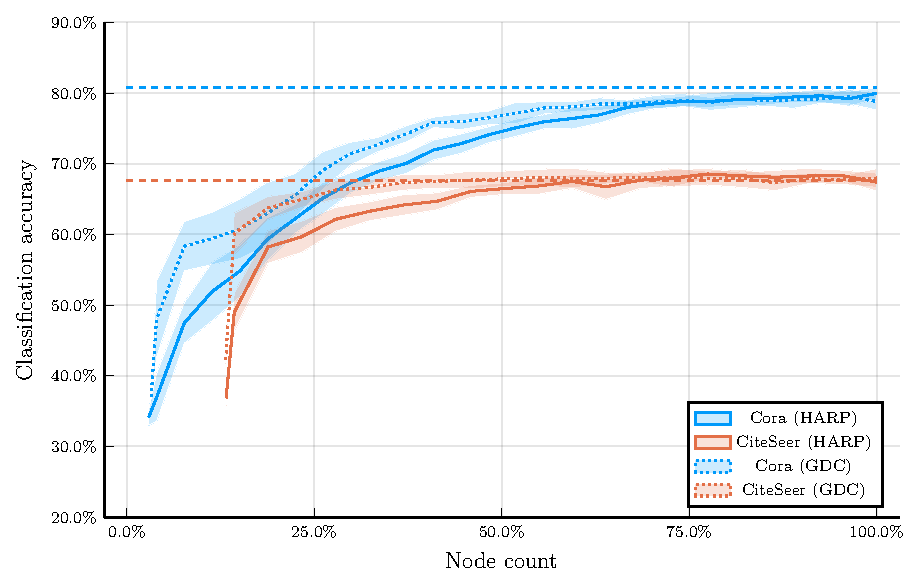
\includegraphics[width=\linewidth]{images/coarsening-algorithms/coarsening-algorithms.pdf}
  \caption{Downstream classifier accuracies at different steps of adaptive prolongation for different coarsening algorithms. Dashed line shows the baseline node2vec model accuracy. The node count is taken relative to the total node count in each dataset. The results are averaged over multiple runs, with the solid line representing the mean and the shaded area denoting one standard deviation.}
  \label{fig:coarsening-algorithms}
\end{figure*}

The behaviour of the models (Figure~\ref{fig:coarsening-algorithms}) again differs substantially between the datasets. As in the previous experiment, the Enzymes dataset contains a lot of noise and generally, the methods behave in a similar manner, retaining decent performance even at the coarsest levels and only improving slightly as more data is available. For both the Cora and the CiteSeer dataset, a clear trend emerges where the GDC coarsening quickly outperforms the original HARP coarsening, with PPR producing better results on Cora under heavy coarsening and both having similar behaviour on CiteSeer. The larger portions of the data the algorithms see, the more the margin shrinks until it vanishes completely. This suggests that the GDC algorithm is able to better preserve the global structure of the graph over successive coarsenings. On the other hand, the evolved coarsening clearly performs the worst, being outperformed by all other methods.

An identical statistical test to the one described in Section~\ref{sec:adaptive-experiments} was carried out for all of the coarsening algorithms. Only the GDC coarsening with the heat kernel rejected the hypothesis that the accuracy is the same from the \( k \)-th decile onwards at the 5\% significance level, for \( k \in \left\{ 1, 2, 3 \right\} \). The Holm-corrected familywise p-values for \( k \in \left\{ 1, 2, 3, 4, 5 \right\} \) were \( 0.019, 0.023, 0.027, 0.071, 0.8 \), respectively. For other algorithms, the hypotheses weren't rejected for any value of \( k \).
